\section*{Continuous Improvement}

The American Society of Quality define Continuous Improvement to be 
\say{The ongoing improvement of products, services or processes through incremental and breakthrough improvements.} \cite{american_society_for_quality_continuous_????}

Continuous Improvement as a concept has existed for a long time. We can find mentions to continuous Improvement in texts dating back to the mid-19th century \cite{schroeder_americas_????}. 

During the Industrial revolution of the mid-19th century workers were often trained not to think but rather just perform just their task. Thus the task of thinking was effectively cut off from the task of doing, which lead to the thinkers not understanding the practical restrictions of the real world and the increasing complexity of the systems \cite{schroeder_americas_????}. The same concept applies even today with software systems. In large organisations developers are often disenfranchised from the decision making process.

This separation of thinkers from the practical implications of real world lead to the development of Continuous improvement which emphasizes a continuous stream incremental innovation \cite{bessant_rediscovering_1994}.

\section*{Continuous Integration}

Continuous improvement incentivizes a structure where hundreds of people are collectively working on the same basic problem set \cite{bessant_rediscovering_1994}. Continuous improvement brings along with it an explosion of ideas and as some of those ideas implemented a surge in the complexity of the system. Such a surge in complexity eventually leads to either the quality or velocity of development to decline \cite{zaytsev_increasing_2013} . 

Continuous integration thus evolved as a mechanism to manage the risk associated with complex software systems \cite{zaytsev_increasing_2013} and  attempts to provide a safety net \cite{fowler_continuous_2006} to developers. 

Though continuous integration doesn't actually fix bugs, it offers a lot of benefits which help in improving the overall quality of the project such as Improved communication, Project predictability and increased developer productivity \cite{sta_ahl_experienced_2013}. So Continuous integration in many ways can be considered a modern method of complexity control \cite{beck_extreme_2000}.

\section*{Software Management and Continuous Integration}

The inherent complexity in software management is best described by the law of leaky abstractions \cite{spolsky_law_2002} which states that all non-trivial abstractions leak to some degree. 

\subsection*{The Law of leaky abstractions}

An abstraction in the context of computers and software refers to a mechanism that tries to hide the complexity of the underlying system while still offering a useful interface to interact effectively with the underlying system. Abstractions are meant to simplify the process of interacting with an inherently complex system by hiding away certain irrelevant details.

Though abstractions vastly simplify interactions with a complex system, the abstractions are still limited by the capabilities of underlying system and  thus some serious failures always trickle up through abstractions and surprise the user in unexpected ways.

\begin{figure*}
  \centering
  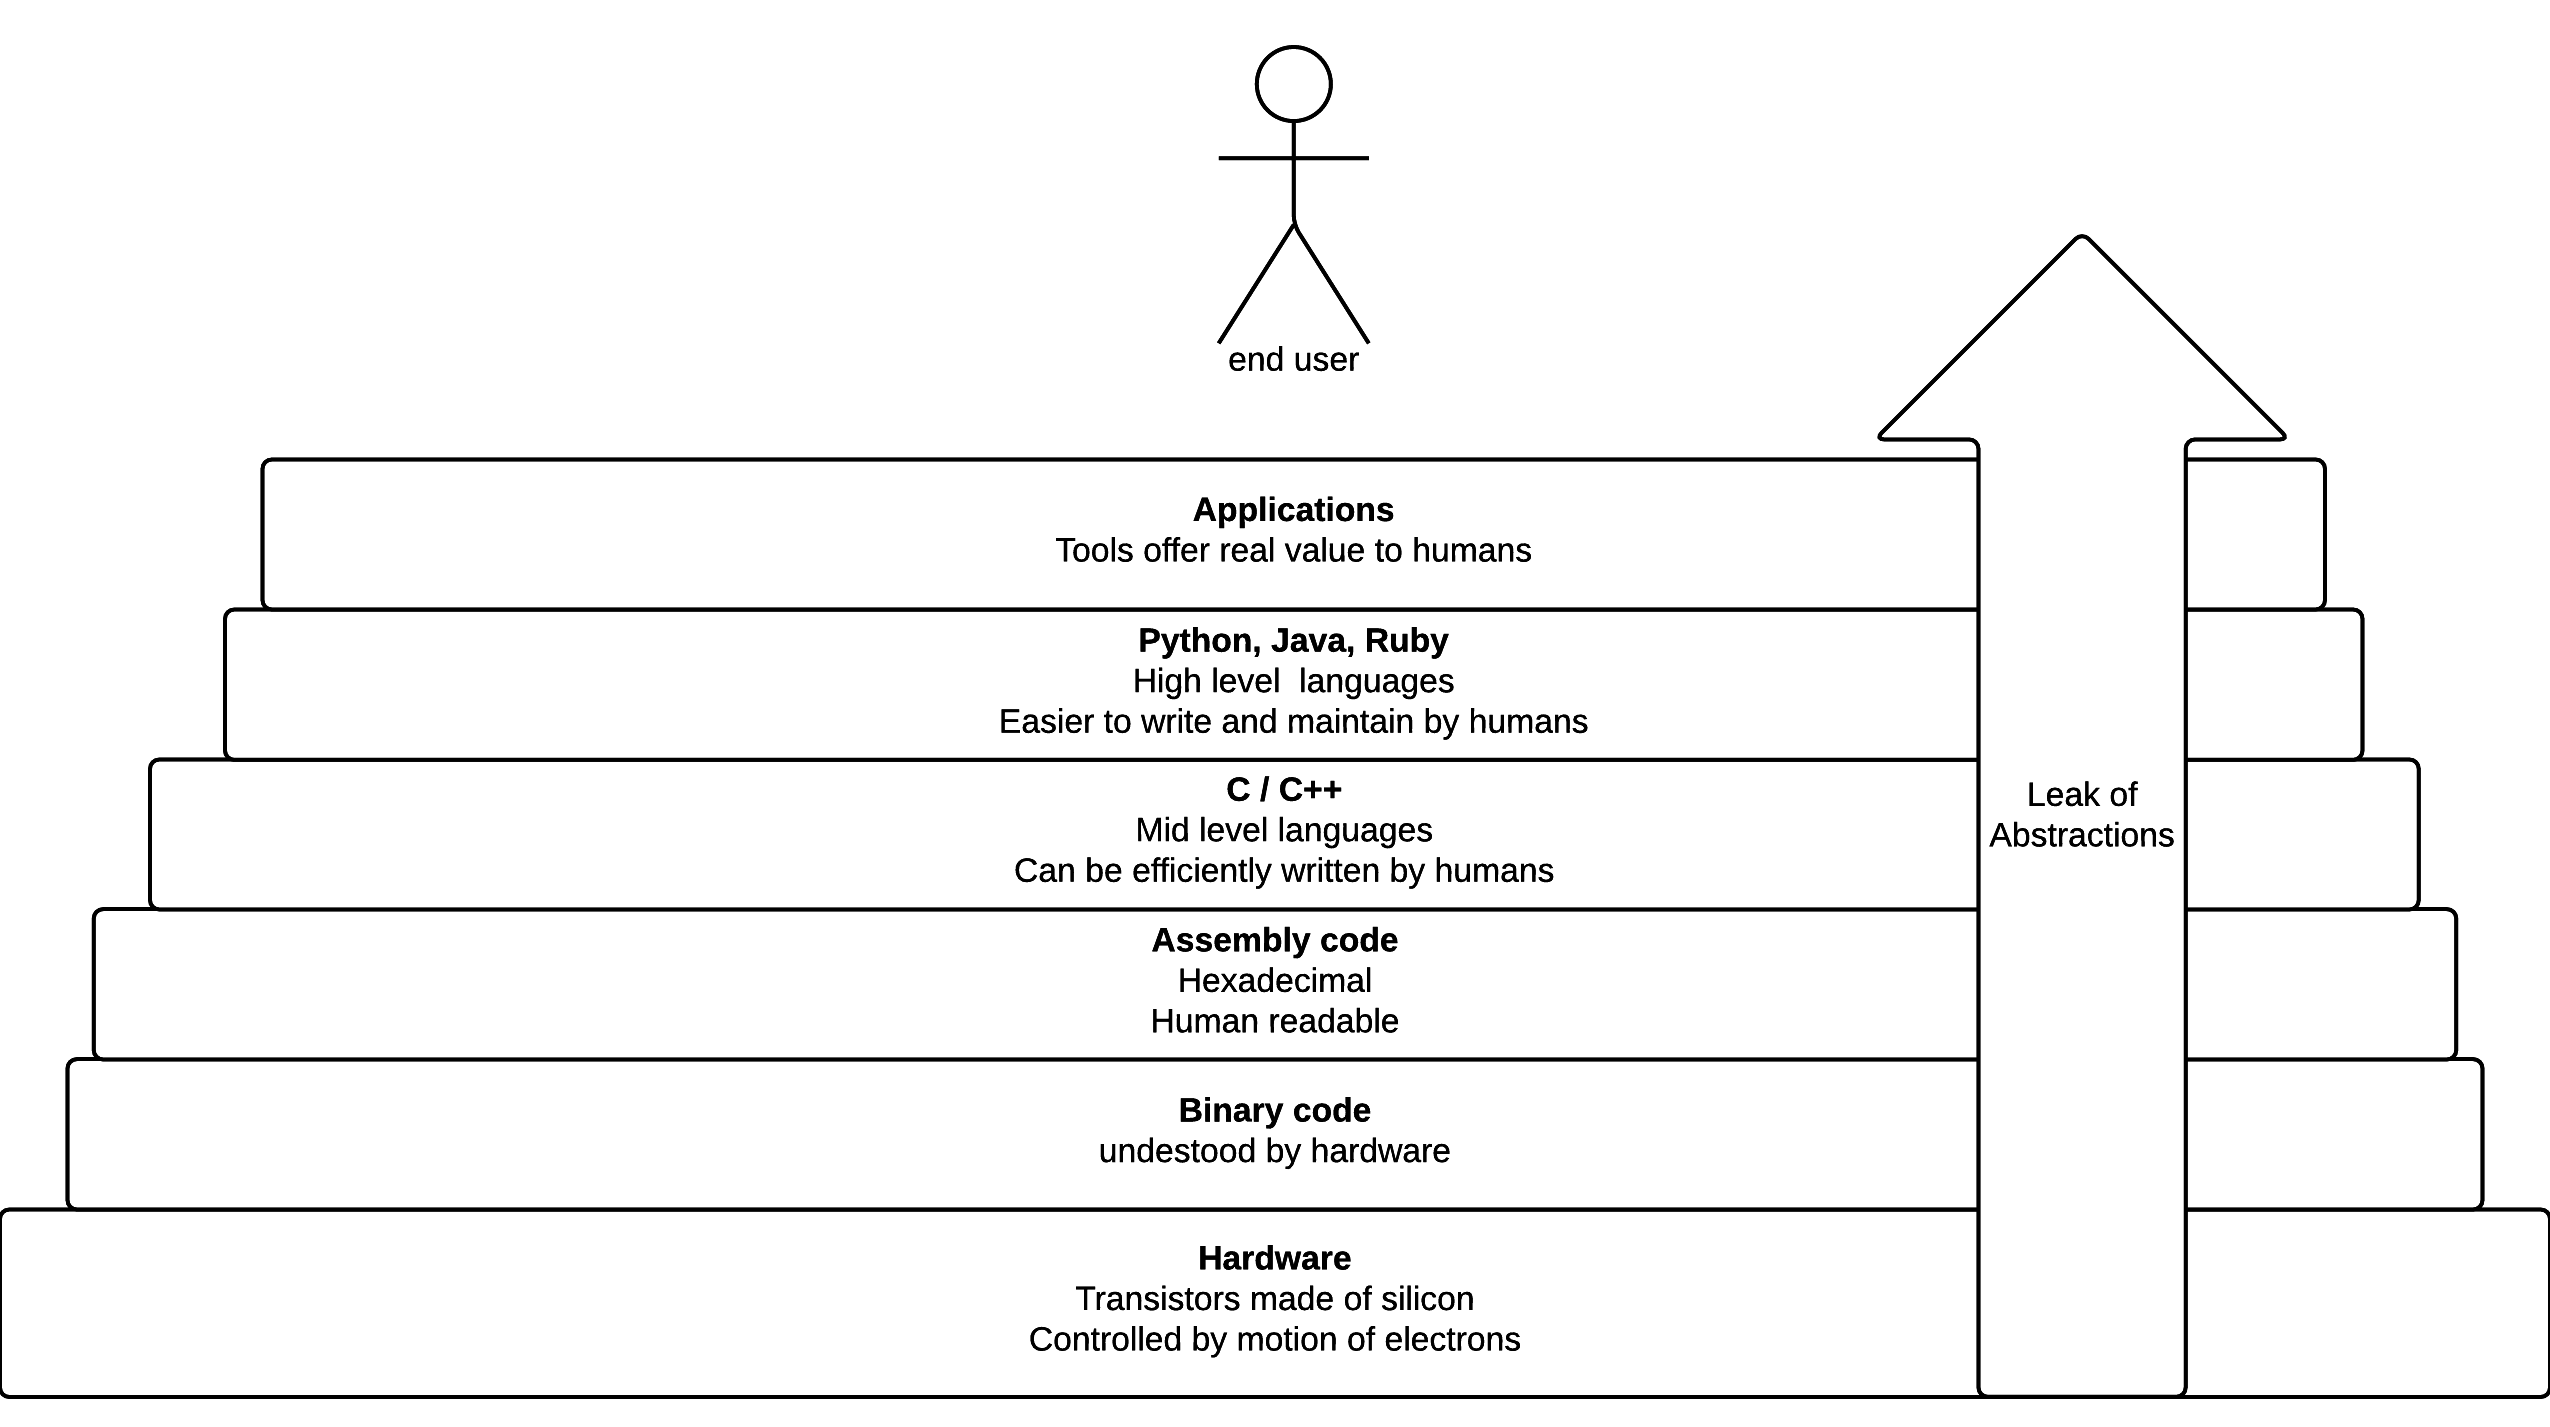
\includegraphics[height=4in]{leakyabstraction}
  \caption{The law of leaky abstraction: All non-trivial abstractions, to some degree, are leaky.}
  \label{leakyabstraction}
\end{figure*}

A classic example of leaky abstractions would be Operating Systems. On the windows operating system any failure in the underlying hardware or its drivers can potentially lead to a BSOD (Blue screen of death) in which the computer displays a cryptic message on a blue screen and prompts the user for action. Though BSOD is a rare occurrence under normal operating conditions, its appearance often perplexes an average user who is unable to make a decision on the next course of action \cite{rosenberg_law_2007}. 

\subsection*{Abstractions in Software Management}

Software Management as a subset of Project management is primarily concerned with balancing the needs of stakeholders with the abilities of developers to deliver value.

Software management practices abstract away the inner workings processes in the organisation. For example Agile methodologies such as Scrum and Kanban are an abstraction which uses best practices from Time management, Team communication, Performance management and Theory of constraints to derive value from developers collaborating within a team. 

Another example of abstraction in Software management in teams would be embracing diversity which is an abstraction over Psychology and Economics to help teams take varied view points on any particular problem. 

\subsection*{CI in Software Management}

Software management is in essence a process which tries to abstract away the chaos of managing an inherently complex task with the help of developers in an ever-evolving environment. As with any non trivial abstraction, software management is leaky and implementing continuous integration into Software management practices could potentially offer benefits similar to software development.